
\documentclass[10pt,a4paper]{article}
\usepackage[T1]{fontenc}
\usepackage{tikz}
\usepackage[margin=1cm]{geometry}
\begin{document}
\subsection*{Initial AVL Tree}
\begin{center}
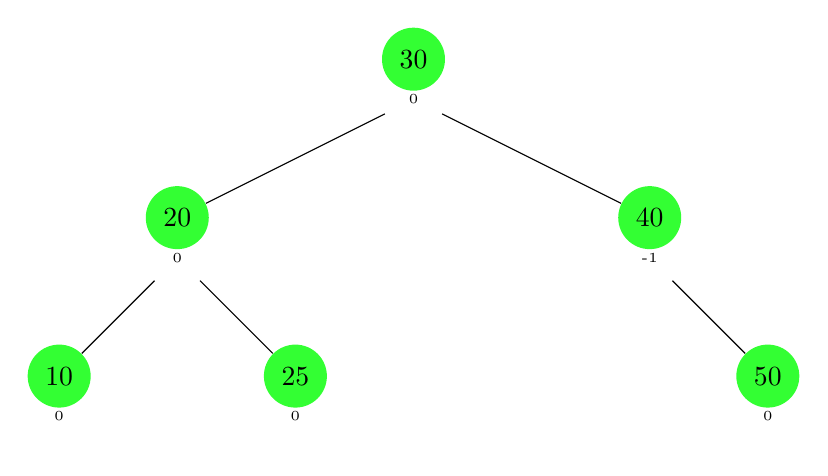
\begin{tikzpicture}[level distance=15mm, sibling distance=20mm]
    \tikzstyle{every node}=[circle,inner sep=1pt, minimum size=8mm]
    \tikzstyle{level 1}=[sibling distance=60mm]
    \tikzstyle{level 2}=[sibling distance=30mm]
    \tikzstyle{level 3}=[sibling distance=15mm]
    \tikzstyle{level 4}=[sibling distance=10mm]
    \node [fill=green!80] {30} node [below=3pt] {\tiny 0} child {node [fill=green!80] {20} node [below=3pt] {\tiny 0} child {node [fill=green!80] {10} node [below=3pt] {\tiny 0} } child {node [fill=green!80] {25} node [below=3pt] {\tiny 0} }} child {node [fill=green!80] {40} node [below=3pt] {\tiny -1} child[fill=none] {edge from parent[draw=none]} child {node [fill=green!80] {50} node [below=3pt] {\tiny 0} }};
\end{tikzpicture}
\end{center}

\subsection*{Step-by-Step Process}
The following figures illustrate the AVL tree at various stages of the insertion and balancing process:


\begin{figure}[h!]
\centering

\begin{minipage}{0.8\textwidth}
    \centering
    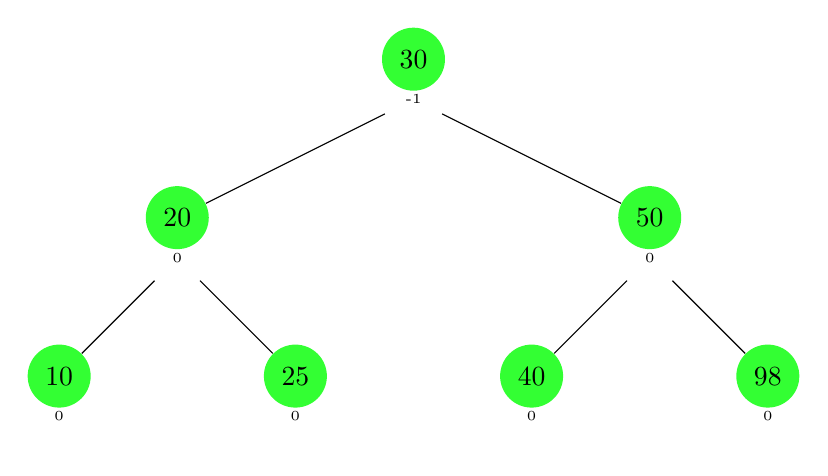
\begin{tikzpicture}[level distance=15mm, sibling distance=20mm]
        \tikzstyle{every node}=[circle,inner sep=1pt, minimum size=8mm]
        \tikzstyle{level 1}=[sibling distance=60mm]
        \tikzstyle{level 2}=[sibling distance=30mm]
        \tikzstyle{level 3}=[sibling distance=15mm]
        \tikzstyle{level 4}=[sibling distance=10mm]
        \node [fill=green!80] {30} node [below=3pt] {\tiny -1} child {node [fill=green!80] {20} node [below=3pt] {\tiny 0} child {node [fill=green!80] {10} node [below=3pt] {\tiny 0} } child {node [fill=green!80] {25} node [below=3pt] {\tiny 0} }} child {node [fill=green!80] {50} node [below=3pt] {\tiny 0} child {node [fill=green!80] {40} node [below=3pt] {\tiny 0} } child {node [fill=green!80] {98} node [below=3pt] {\tiny 0} }};
    \end{tikzpicture}
    \caption{Step 1}
\end{minipage}
\vspace{1cm}

\begin{minipage}{0.8\textwidth}
    \centering
    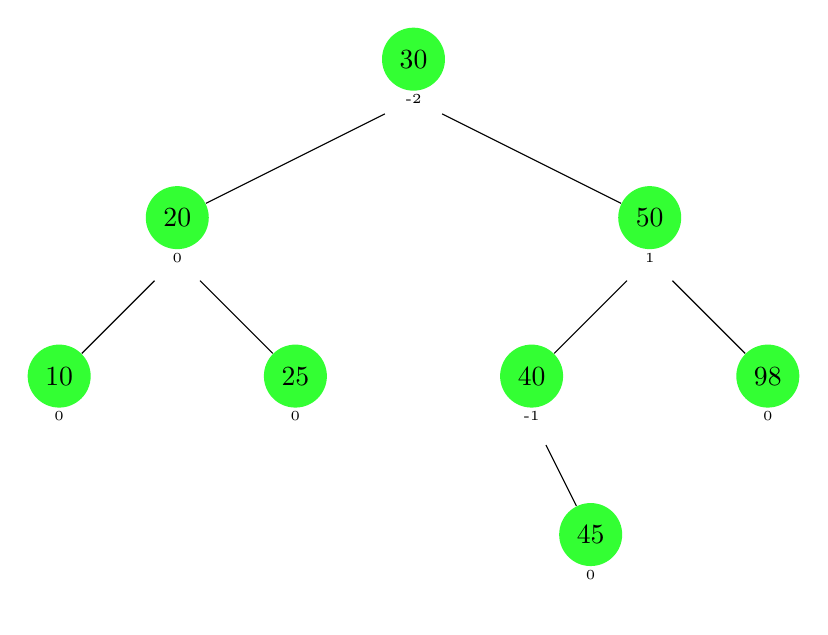
\begin{tikzpicture}[level distance=15mm, sibling distance=20mm]
        \tikzstyle{every node}=[circle,inner sep=1pt, minimum size=8mm]
        \tikzstyle{level 1}=[sibling distance=60mm]
        \tikzstyle{level 2}=[sibling distance=30mm]
        \tikzstyle{level 3}=[sibling distance=15mm]
        \tikzstyle{level 4}=[sibling distance=10mm]
        \node [fill=green!80] {30} node [below=3pt] {\tiny -2} child {node [fill=green!80] {20} node [below=3pt] {\tiny 0} child {node [fill=green!80] {10} node [below=3pt] {\tiny 0} } child {node [fill=green!80] {25} node [below=3pt] {\tiny 0} }} child {node [fill=green!80] {50} node [below=3pt] {\tiny 1} child {node [fill=green!80] {40} node [below=3pt] {\tiny -1} child[fill=none] {edge from parent[draw=none]} child {node [fill=green!80] {45} node [below=3pt] {\tiny 0} }} child {node [fill=green!80] {98} node [below=3pt] {\tiny 0} }};
    \end{tikzpicture}
    \caption{Step 2}
\end{minipage}
\vspace{1cm}

\begin{minipage}{0.8\textwidth}
    \centering
    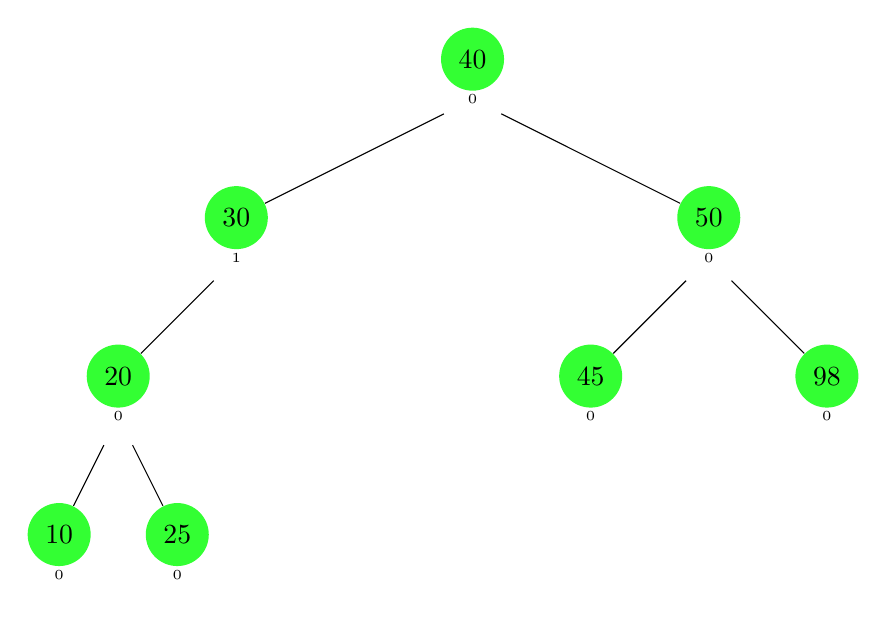
\begin{tikzpicture}[level distance=15mm, sibling distance=20mm]
        \tikzstyle{every node}=[circle,inner sep=1pt, minimum size=8mm]
        \tikzstyle{level 1}=[sibling distance=60mm]
        \tikzstyle{level 2}=[sibling distance=30mm]
        \tikzstyle{level 3}=[sibling distance=15mm]
        \tikzstyle{level 4}=[sibling distance=10mm]
        \node [fill=green!80] {40} node [below=3pt] {\tiny 0} child {node [fill=green!80] {30} node [below=3pt] {\tiny 1} child {node [fill=green!80] {20} node [below=3pt] {\tiny 0} child {node [fill=green!80] {10} node [below=3pt] {\tiny 0} } child {node [fill=green!80] {25} node [below=3pt] {\tiny 0} }} child[fill=none] {edge from parent[draw=none]}} child {node [fill=green!80] {50} node [below=3pt] {\tiny 0} child {node [fill=green!80] {45} node [below=3pt] {\tiny 0} } child {node [fill=green!80] {98} node [below=3pt] {\tiny 0} }};
    \end{tikzpicture}
    \caption{Step 3}
\end{minipage}
\vspace{1cm}

\end{figure}
\newpage

\end{document}
